\documentclass[11pt, oneside]{article} 
\usepackage{geometry}
\geometry{letterpaper} 
\usepackage{graphicx}
	
\usepackage{amssymb}
\usepackage{amsmath}
\usepackage{parskip}
\usepackage{color}
\usepackage{hyperref}

\graphicspath{{/Users/telliott/Github/calculus_book/png/}}
% \begin{center} \includegraphics [scale=0.4] {gauss3.png} \end{center}

\title{Quadrature}
\date{}

\begin{document}
\maketitle
\Large
\label{sec:quad}

Let's talk about Archimedes, and parabolas.

Here is a figure from wikipedia, showing a parabola and a chord of the parabola, which might be drawn between any two points.  A triangle is constructed from the chord in the following way:  the point dividing the horizontal distance in half is found and that is used for the x-value of the third point.

\begin{center} 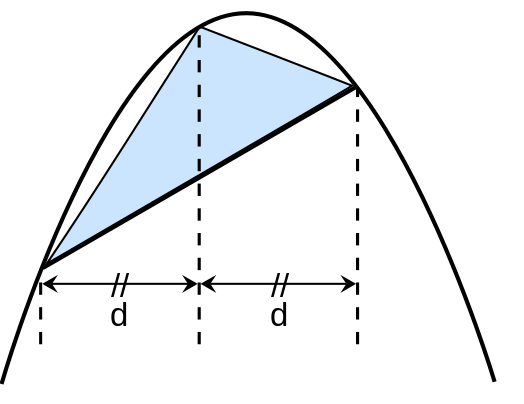
\includegraphics [scale=0.35] {para_tri.png} \end{center}
The Greek genius Archimedes showed that the total area underneath the curve, between the two outside vertices of the triangle, is $4/3$ times the area of the triangle shown in blue. The method he used is called the "quadrature of the parabola" and it is (from our modern perspective) a relatively simple though still revolutionary idea.

One very interesting consequence is that the slope of the tangent to the parabola at this midway point is equal to the slope of the chord.

The general equation of a parabola is
\[ y = ax^2 + bx + c \]
But for any given parabola, we can translate it to the origin and the parabola at the origin with the same shape is
\[ y = ax^2 \]
This can be demonstrated by completing the square.

If we pick two points on the parabola at $x=u$ and $x=v$, then the corresponding coordinates are
\[ P = (u, \ au^2) \]
\[ Q = (v, \ av^2) \]
\begin{center} 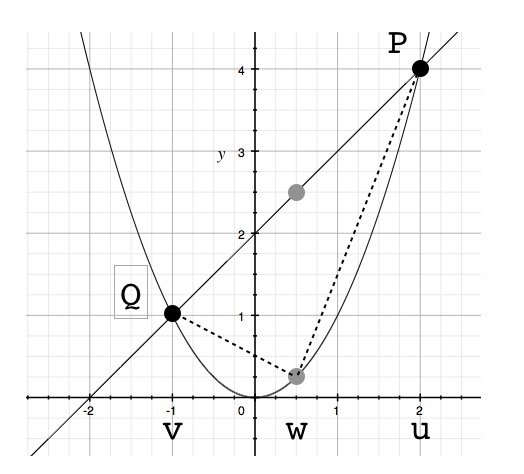
\includegraphics [scale=0.45] {para_tri2.png} \end{center}
$P$ is the right-hand point in the figure.  Let us say that $au^2 > av^2$ and  
and the slope $m$ of the chord that connects them is
\[ m =\frac{au^2 - av^2}{u - v} = \frac{a(u^2-v^2)}{u - v} = \frac{a(u-v)(u+v)}{u - v} \]
so
\[ m = a(u+v) \]
We can see that this formula gives the correct answer for $u = - v$, since the slope at the vertex is $0$.  Now label the midpoint $x=w$
\[ w = \frac{1}{2}(u + v) \]
And the slope at $w$ (from calculus) is
\[ f'(w) = 2aw = = 2a \ \frac{1}{2}(u+v) = a(u + v) \]
So the proposition is correct.

\subsection*{Quadrature}
Another interesting thing about this figure is that the area of the triangle can be found from the length of the vertical coming down from the top.
\begin{center} 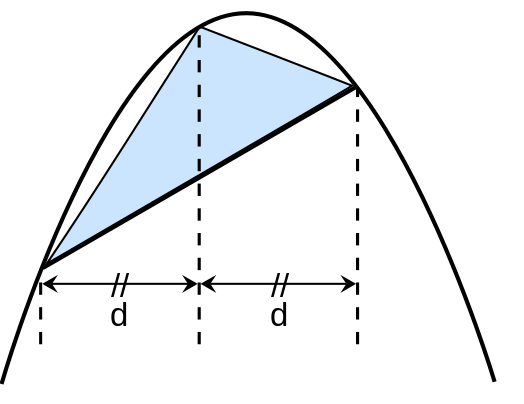
\includegraphics [scale=0.4] {para_tri.png} \end{center}

If we simply turn the graph sideways in our mind, then the two small triangles share the part of this line within the blue region, which is their "base", $b$.  And they both have "height" $d$, since $w$ was chosen as half way between $u$ and $v$, so their areas are equal, and the total area of the two together is
\[ A = bd \]
We want to find an expression for the area only in terms of $u$ and $v$ (no $b$ or $d$).  Let's look at the second version of the figure again below.  

To repeat, what we found above is that the slope at the point on the parabola corresponding to $x=w$ is equal to the slope of the line that connects $v$ and $u$, and more important to us now, that the area of the combined triangle (vertices $u,v,w$) is
\[ A = (u-w) \ b = \frac{1}{2} (u-v) \ b \]
where $b$ is the distance parallel to the $y$-axis between the two points marked in gray.  
\begin{center} 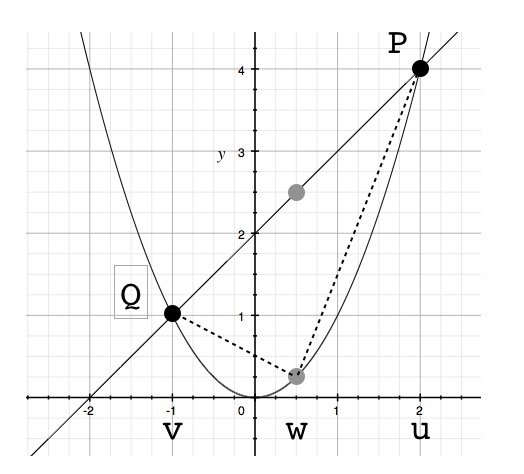
\includegraphics [scale=0.4] {para_tri2.png} \end{center}
The length of the "base" $b$ is the average of the y-values for $x=u$ and $x=v$, minus $aw^2$.
\[ b = \frac{1}{2}(au^2+av^2) - aw^2 \]
and from before
\[ w = \frac{1}{2}(u+v) \]
so we have
\[ b = \frac{1}{2}(au^2+av^2) - a\ [\ \frac{1}{2}(u+v)\ ]^2 \]
Factor out $a/4$
\[ = \frac{1}{4} a\ [\ 2u^2 + 2v^2 - (u+v)^2 \ ] \ \]
\[ = \frac{1}{4} a\ [\ 2u^2 + 2v^2 - u^2 - 2uv - v^2 \ ] \ \]
\[ = \frac{1}{4} a\ [\ u^2 - 2uv + v^2 \ ] \  \]
\[ b = \frac{1}{4} a\ (u-v)^2 \]
The area is
\begin{equation}
\boxed{A = bd = \frac{1}{8} a\  (u-v)^3}
\end{equation}

\subsection*{check}
We'll check three cases to see if this makes sense.  First if 
\[ u = v \]
then the area is zero and $w=u=v$, so that's good.  Second, if 
\[ u = -v \]
then
\[ A = \frac{1}{8} a\ (u-v)^3  = \frac{1}{8} a\  (2u)^3  = au^3 \]
We compare this result with a direct computation by geometry.  In the figure we have two symmetric triangles with individual area 
\[ \frac{1}{2} u \ au^2 \]
The total area is twice that, so it checks.  Finally, suppose we have $v = 0$
\[ A = \frac{1}{8} a\  (u-v)^3 \]
This one is harder to see, but we have that 
\[ d = \frac{1}{2} (u-v) = \frac{1}{2}u \]
$b$ is the distance between the average y-value which is $(1/2)au^2$ and $aw^2 = a(u/2)^2$
\[ b = a\   (\frac{1}{2}u)^2 - \frac{1}{2}\ [\ au^2-0\ ]\  = \ \frac{1}{4}a \ u^2 \]
\[ A = bd = \frac{1}{8}au^3 \]
so they all check.

\subsection*{Quadrature of the parabola}
\begin{center} 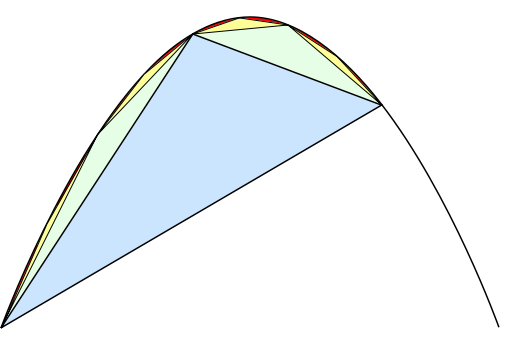
\includegraphics [scale=0.4] {para_tri3.png} \end{center}
The reason for the whole preceding argument is this.  The area formula is
\[ A = bd = \frac{1}{8} a\ (u-v)^3 = k(u-v)^3, \ \ k = const \]
It is solely a function of $u-v$.  Suppose we draw two new triangles (in light green, above).  For each of these triangles the distance between the new vertices is one-half what we had before.  So everything that we have for the big blue triangle is also true for these two new ones, just adjusted by a factor of $u'-v' = (1/2)(u-v$).

What this means is that the area of each light green triangle is in the ratio to the blue one of $(1/2)^3 = 1/8$.  But there are two of these new triangles, so the new area we added is in the ratio $1/4$.

Suppose we do it again, constructing the yellow triangles.  The new area of each is in the ratio $(1/4)^3 = 1/64$ but there are now $4$ of these yellow triangles so the total area is in the ratio $1/16 = (1/4)^2$

If we call the area of the original triangle $T$, that of the blue plus the light green is

\[ A = T + \frac{1}{4} T \]
and with the addition of the yellow it is

\[ A = T + \frac{1}{4} T  + \frac{1}{16} T \]
so, as an infinite series it is

\[ A = T(1 + \frac{1}{4} + \frac{1}{16} + \cdots ) \]

Here is Archimedes' proof that the sum of this series (not counting the first term) is $1/3$.  

\begin{center} 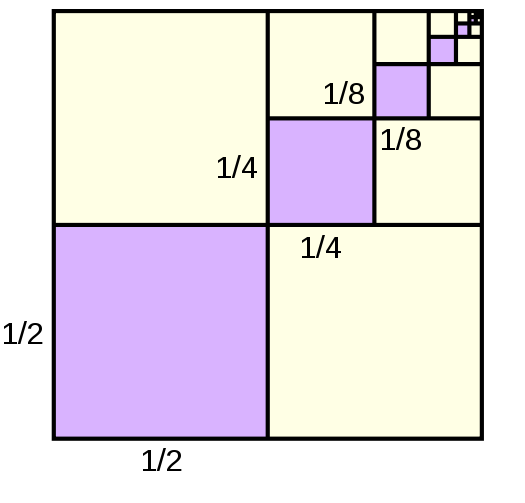
\includegraphics [scale=0.4] {para_series_sum.png} \end{center}
So the total is $4/3$, and the complete area under the parabola is $4/3$ the area of the triangle drawn as we described!

This called the "method of exhaustion", and not just because it's a lot of work.


\end{document}